\chapter{$\infty$-范畴的语言}

% 简要介绍无穷范畴的历史?

\philoquote{The traditional way in the literature to provide foundations (for higher category theory) is via the theory of \emph{quasi-categories}, which in turn rests on set theory. While this can be done, the language of set theory is simply not very adequate to model homotopical notions, ...}{Denis-Charles Cisinski, \cite{FHC}}

%像许多 $\infty$-范畴论的文献一样, 本书使用 $\infty$-范畴的一种公理化语言. 我们不是从 $\infty$-范畴的任何一种定义 (或模型) 出发, 而是以公理的形式刻画期望中 $\infty$-范畴的行为. %这样我们可以获得\emph{模型无关} (model-independent) 的结果.



%同伦类型论 (Homotopy Type Theory, HoTT) 提供了 $\infty$-群胚的语言. 我们也可以用一种类似的类型论来谈论 $\infty$-范畴.
% https://arxiv.org/pdf/1705.07442

$\infty$-范畴作为一种模糊的概念已经存在很久. 然而在数学上, $\infty$-范畴没有确切的定义. 在集合论的基础上, 为了逼近心目中那个完美的概念, 人们建立了 $\infty$-范畴各种各样的\emph{模型}. 最著名的模型是由 Andr\'e Joyal 提出, Jacob Lurie \cite{HTT} 发展的基于单纯集的\emph{拟范畴} (quasicategory). 每一种模型都有人为的成分, 而模型之间的等价性是非常不平凡的问题. %在模型中手动构造任何函子都是几乎不可能的.

设想有一个称为 ``\emph{无穷范畴国}'' 的天国乐园, 其国民使用 $\infty$-范畴内蕴的语言作为母语, 他们谈笑之间就可以完成凡人不可想象的工作. 在地上, 说着集合论语言的人们用尽力气, 搭建了通往天国的阶梯, 到访了天国. 但人们发现, 为了理解无穷范畴中任何一件稀松平常的小事, 都要耗费数倍的精力. 地上的人们终于意识到, 语言不通是他们面前最大的阻碍. 要想像母语者那样自如地使用无穷范畴, 就必须抛弃集合论的某些思维, 甚至经典逻辑的一些信条.

能代替集合论成为数学基础, 并且适合于 $\infty$-范畴理论的一种语言是\emph{同伦类型论} (homotopy type theory, HoTT) \cite{hottbook}, 同伦类型论以基本概念 ``类型'' 为 $\infty$-群胚提供了语法, 并且自身包含了一整套推理系统; 理解这种语言对理解 $\infty$-范畴理论中的许多现象有很大的帮助, 因此我们在第 0 节简要介绍之. Emily Riehl 与 Michael Shulman \cite{riehl2023typetheorysyntheticinftycategories} 使用 HoTT 的变种 ``有向类型论'' (directed type theory) 建立了一种综合 $\infty$-范畴理论, Matthew Weaver 和 Daniel Licata 采用的另一变种 ``立方类型论'' (cubical type theory) 也在这个领域展现出一些优势.


%从地上通向天国的阶梯

\setcounter{section}{-1}
\section{同伦类型论基础}

本节介绍的同伦类型论仅供 $\infty$-群胚的理解所需, 因此我们不会使用最正式的语言 (对此有需要的读者可参见 \cite{hottbook} 附录 A).

\begin{axiom}
	{(类型, 对象)}
	同伦类型论有两个基本概念, \emph{类型} (type) 与\emph{对象} (object);
	有一个基本\emph{断言} (judgement)
	\[
	a : A
	\]
	表示 ``对象 $a$ 具有类型 $A$''.
\end{axiom}

\begin{remark}
	{}
	在同伦类型论中, 类型的直观是空间, 而对象是空间中的点.
	此外, \emph{断言}和\emph{命题}是不同的两种东西. 后面我们会介绍命题是一种特殊的类型.
\end{remark}

\begin{axiom}
	{(宇宙)}
	有一个类型 $\mathcal U$ 称为\emph{宇宙},
	我们将用陈述 $$A : \mathcal U$$
	表示 ``$A$ 是类型''.
\end{axiom}

\newcommand{\refl}{\mathsf{refl}}

\begin{axiom}
	{(等式类型)}
	对于类型 $A : \mathcal U$ 的两个对象 $a,b:A$, 有一个类型
	\[
	a=_Ab, \quad\text{或简记为}\quad a=b,
	\]
	称为\emph{等式类型} (identity type).
	
	对每个对象 $a : A$ 有一个对象
	\[
	\refl_a : a=a,
	\]
	称为\emph{自反} (reflexivity).
\end{axiom}

\begin{remark}
	{}
	在同伦类型论中, 两个对象的相等不是一个\emph{断言}, 也不是一个\emph{命题}, 而是一个新的\emph{类型}.
	这就如同一个空间中两个点之间的道路构成一个新的空间,
	又如同 $\infty$-群胚中两个对象之间的态射构成一个新的 $\infty$-群胚;
	这个新的类型包含的同伦信息不止于空或非空.
	
	有时我们也需要以断言的形式表达两个对象依定义相等. 请注意等式类型与依定义相等的区别.
\end{remark}

\begin{axiom}
	{(依定义相等)}
	同伦类型论有一个基本断言
	\[
	a\equiv b : A
	\]
	表示 ``类型 $A$ 的两个对象 $a$ 与 $b$ 依定义相等''.
\end{axiom}

\begin{axiom}
	{(函数类型)}
	对于两个类型 $A,B : \mathcal U$, 有一个类型 $$(A\to B) : \mathcal U,$$
	称为\emph{函数类型} (function type).
	对 $f\colon A\to B$ 以及 $a : A$ 有 $f(a) : B$.
	
	对于含有变量 $x$ 的表达式 $\Phi$, 若 $x : A$ 时有 $\Phi : B$,
	则可定义所谓 \emph{$\lambda$-抽象} (abstraction)
	\[
	(\lambda x.\Phi) : A \to B,
	\]
	此时对于 $a : A$, 记 $\Phi'$ 为将表达式 $\Phi$ 中所有 $x$ 替换为 $a$ 的结果,
	则有
	$$(\lambda x.\Phi)(a) \equiv \Phi'.$$
	对每个 $f \colon A\to B$ 有
	$$
	f \equiv (\lambda x.f(x)).
	$$
\end{axiom}

\begin{example}
	{(依值类型)}
	一个函数 $B\colon A \to \mathcal U$ 称作一个\emph{类型族} (type family) 或一族\emph{依值类型} (dependent type),
	即对类型 $A$ 的每个对象 $a : A$ 都有一个类型 $B(a) : \mathcal U$.
\end{example}

\newcommand{\pr}{\mathsf{pr}}

\begin{axiom}
	{(乘积类型)}
	对于两个类型 $A,B : \mathcal U$ 有一个类型 $$(A\times B) : \mathcal U,$$
	称为\emph{乘积类型} (product type),
	其对象形如 $(a,b)$, $a:A$, $b:B$.
	有两个函数 $$\pr_1\colon A\times B\to A,\quad
	\pr_2\colon A\times B\to B,$$
	以及断言
	\[
	\pr_1((a,b)) \equiv a,\quad
	\pr_2((a,b)) \equiv b.
	\]
\end{axiom}

\begin{axiom}
	{(依值和类型)}
	对于类型 $A : \mathcal U$ 以及依值类型 $B : A \to \mathcal U$,
	有一个类型
	\[
	\sum_{x : A} B(x),
	\]
	称为\emph{依值和类型} (dependent sum type),
	其对象形如 $(a,b)$, $a:A$, $b:B(a)$.
	有一个函数 $$\pr_1\colon \Big(\sum_{x : A} B(x)\Big) \to A.$$
\end{axiom}

\begin{axiom}
	{(依值积类型)}
	对于类型 $A : \mathcal U$ 以及依值类型 $B : A \to \mathcal U$,
	有一个类型
	\[
	\prod_{x : A} B(x),
	\]
	称为\emph{依值积类型} (dependent product type),
	对于表达式 $\Phi : B(x)$,
	有 $$\lambda x.\Phi : \prod_{x:A} B(x).$$
	对于 $f:\prod_{x:A} B(x)$ 以及 $a:A$ 有 $f(a) : B(a)$, 且有断言
	$f(a) \equiv \Phi'$, $\Phi'$ 为将 $\Phi$ 中所有 $x$ 替换为 $a$ 得到的表达式.
\end{axiom}



\begin{definition}
	{(命题是类型)}
	同伦类型论中的\emph{命题}是\emph{类型}.
	证明一个命题就是构造一个类型的对象.
	\begin{center}
		\begin{tabular}{ll}
			命题 & 类型 \\
			\hline
			$A$ 且 $B$ & $A\times B$ \\
			$A$ 或 $B$ & $A+B$\\
			若 $A$ 则 $B$ & $A\to B$\\
			非 $A$ & $A\to 0$\\
			$A$ 当且仅当 $B$ & $(A\to B)\times (B\to A)$\\
			对任意 $x:A$, $P(x)$ & $\prod_{x:A}P(x)$\\
			存在 $x:A$, $P(x)$ & $\sum_{x : A} P(x)$
		\end{tabular}
	\end{center}
\end{definition}

\subsection{集合, 逻辑与截断性}

\newcommand{\isprop}{\mathsf{isProp}}
\newcommand{\isset}{\mathsf{isSet}}
\newcommand{\iscontr}{\mathsf{isContr}}

\begin{definition}
	{(命题)}
	对于类型 $P$ 定义
	\[
	\isprop(P) :\equiv \prod_{x,y : P} (x=y).
	\]
	若 $\isprop(P)$ 有对象, 则称 $P$ 为\emph{命题}.
\end{definition}

\begin{remark}
	{(排中律)}
	在同伦类型论中, 排中律可定义为
	\[
	\mathsf {LEM} :\equiv \prod_{A : \mathcal U}\big(
	\isprop(A) \to (A + \neg A)
	\big).
	\]
	构造主义告诉我们许多的数学不需要排中律 (但这不代表我们需要否认排中律).
\end{remark}

\begin{definition}
	{(集合)}
	对于类型 $S$ 定义
	\[
	\isset(S) :\equiv \prod_{x,y : S}\isprop(x=y).
	\]
	若 $\isset(S)$ 有对象, 则称 $S$ 为\emph{集合}.
\end{definition}

\begin{definition}
	{(命题截断)}
	对于类型 $A$ 有一个类型 $\|A\|$, 称为其\emph{命题截断} (propositional truncation),
	\begin{itemize}
		\item 对任意 $a:A$ 有 $|a|:\|A\|$;
		\item 对任意 $x,y:\|A\|$ 有 $x=y$.
	\end{itemize}
\end{definition}

\begin{definition}
	{(可缩类型)}
	对于类型 $A$ 定义
	\[
	\iscontr(A) :\equiv \sum_{a : A} \prod_{x : A} (a=x).
	\]
\end{definition}

\begin{remark}
	{}
	按朴素的理解, $\iscontr(A)$ 似乎表达的是连通性: ``存在点 $a:A$, 使得对任意点 $x:A$, 都有一条 $a$ 到 $x$ 的路径.''
	但在同伦类型论中, 依值积类型 (全称量词) 的证据需要某种连续性, 直观上需要这条 $a$ 到 $x$ 的路径随 $x$ ``连续变化'', 于是整个命题描述的就不仅是连通性, 而是可缩性.
\end{remark}

\section{基本概念}

本章不会给出无穷范畴的定义. 相反, 我们描述在无穷范畴的语言中, \emph{我们希望能说什么}, 并以公理的形式刻画期望中 $\infty$-范畴的行为. 请注意本章介绍的不是一个完整的 $\infty$-范畴理论, 这些公理不一定出现在最终 ``完美'' 的理论中, 甚至我们不知道那样一个理论是否存在或唯一.

\begin{axiom}
	{($\infty$-范畴)}
	我们要谈论一些对象, 称之为 \emph{$\infty$-范畴} $\mathcal C,\mathcal D,\mathcal E,\cdots$.
	我们还要谈论这些对象之间的\emph{函子} $f\colon \mathcal C\to \mathcal D$, $g\colon \mathcal D\to\mathcal E$ 等等.
\end{axiom}

% 无穷范畴的等价是什么? 伴随等价还是朴素等价?

% 要不要先描述无穷群胚? 我觉得是合理的, 按照 r 递增的顺序来描述 (∞,r)-范畴.

% 澄清 "唯一" 的概念.

\begin{axiom}
	{(一些重要的 $\infty$-范畴)}
	存在如下的 $\infty$-范畴:
	\begin{itemize}
		\item \emph{始 $\infty$-范畴}, 记作 $0$ (或 $\varnothing$), 满足从 $0$ 到任何 $\infty$-范畴 $\mathcal C$ 有唯一的函子;
		\item \emph{终 $\infty$-范畴}, 记作 $1$, 满足从任何 $\infty$-范畴 $\mathcal C$ 到 $1$ 有唯一的函子;
		\item 对任何两个 $\infty$-范畴 $\mathcal C,\mathcal D$, 存在两者的\emph{积} $\mathcal C\times \mathcal D$,
		使得对另一个 $\infty$-范畴 $\mathcal E$,
		一个函子 $\mathcal E\to\mathcal C\times\mathcal D$ 等同于两个函子 $\mathcal E\to\mathcal C$, $\mathcal E\to\mathcal D$;
		\item 对任何两个 $\infty$-范畴 $\mathcal C,\mathcal D$, 存在两者的\emph{和} $\mathcal C + \mathcal D$,
		使得对另一个 $\infty$-范畴 $\mathcal E$,
		一个函子 $\mathcal C + \mathcal D \to \mathcal E$ 等同于两个函子 $\mathcal C \to \mathcal E$, $\mathcal D \to \mathcal E$;
		\item 对任何两个 $\infty$-范畴 $\mathcal C,\mathcal D$, 有\emph{函子范畴} $\mathsf {Fun}(\mathcal C,\mathcal D)$,
		也记作 $\mathcal D^{\mathcal C}$, 使得对另一个 $\infty$-范畴 $\mathcal E$,
		函子 $\mathcal E\to \mathcal D^{\mathcal C}$ 等同于函子 $\mathcal E\times\mathcal C \to \mathcal D$;
	\end{itemize}
\end{axiom}

\begin{axiom}
	[label={regular-category-as-infinity-category}]
	{($1$-范畴视为 $\infty$-范畴)}
	每个普通范畴 (即 $1$-范畴) 都可以视为 $\infty$-范畴. 普通范畴之间的函子也可以视为对应的 $\infty$-范畴之间的函子.
	普通范畴的和与积就是它们作为 $\infty$-范畴的和与积.
\end{axiom}

\begin{axiom}
	{(对象, 态射)}
	$\infty$-范畴 $\mathcal C$ 的\emph{对象}等同于函子 $1\to \mathcal C$.
	两个对象之间的态射等同于函子 $\{*\to *\}\to \mathcal C$, 其中 $\{*\to *\}$ 视为 $\infty$-范畴 (公理 \ref{regular-category-as-infinity-category}).
	称函子范畴 $\mathcal C^{\{*\to *\}}$ 为\emph{箭头范畴}, 也简记为 $\mathcal C^\rightarrow$.
\end{axiom}

\section{$\infty$-范畴中的结构与性质}

\subsection{连通性与截断性}

% HoTT?

\begin{definition}
	{($n$-截断 $\infty$-群胚, $n$-群胚)}
	设 $n\geq -1$ 为整数. 称一个 $\infty$-群胚 $X$  \emph{$n$-截断} (或称其为 \emph{$n$-群胚}) 是指其所有大于 $n$ 阶的同伦群 $\pi_k(X)\,(k>n)$ 均平凡.
\end{definition}

\begin{definition}
	{($n$-群胚, 等价定义)}
	设 $n\geq -1$ 为整数. 称一个 $\infty$-群胚 $X$  \emph{$n$-截断}是指 $X$ 为关于 $\{S^{n+1}\to *\}$ 的局部对象.
\end{definition}

\begin{example}
	{(低维群胚的例子)}
	在同伦等价的意义下,
	\begin{itemize}
		\item $(-2)$-群胚是一个点.
		\item $(-1)$-群胚是空集或一个点.
		\item $0$-群胚是集合, 也即离散群胚.
	\end{itemize}
\end{example}

\subsection{$n$-范畴}

\begin{definition}
	[label={local-objects-infinity-category}]
	{(局部对象)}
	设 $\mathcal C$ 为 $\infty$-范畴, $S$ 为 $\mathcal C$ 中一族态射的集合, 称 $\mathcal C$ 的对象 $x$ 为 \emph{$S$-局部对象}是指对 $S$ 中任意态射 $f\colon a\to b$,
	\[
	f^*\colon \operatorname{Hom}_{\mathcal C}(b,x) \to \operatorname{Hom}_{\mathcal C}(a,x)
	\]
	为 $\infty$-群胚的等价.
	%这是定义 \ref{local-objects} 在 $\infty$-范畴中的类比.
\end{definition}

\begin{definition}
	{(球面)}
	归纳定义 $\infGpdinfcat$ 的 \emph{$n$ 维球面} $S^n\,(n\geq -1)$ 如下:
	\begin{itemize}
		\item $S^{-1}=\varnothing$;
		\item 对 $n\geq -1$, $S^{n+1}$ 是如图所示的推出.
		% https://q.uiver.app/#q=WzAsNCxbMCwwLCJTXntufSJdLFswLDEsIioiXSxbMSwwLCIqIl0sWzEsMSwiU157bisxfSJdLFswLDFdLFsxLDNdLFswLDJdLFsyLDNdXQ==
	\end{itemize}
	\vspace{-6.5em}
	\begin{flushright}
		$\begin{tikzcd}[ampersand replacement=\&,column sep=small]
			{S^{n}} \& {*} \\
			{*} \& {S^{n+1}}
			\arrow[from=1-1, to=2-1]
			\arrow[from=2-1, to=2-2]
			\arrow[from=1-1, to=1-2]
			\arrow[from=1-2, to=2-2]
		\end{tikzcd}$
	\end{flushright}
\end{definition}

\begin{definition}
	{($n$-群胚)}
	对整数 $n\geq -2$, 定义 \emph{$n$-群胚}为 $\infGpdinfcat$ 中关于 $\{S^{n+1}\to *\}$ 的局部对象 (定义 \ref{local-objects-infinity-category}).
\end{definition}



\subsection{东西, 结构, 性质}

\subsection{伴随}

%在定义极限和余极限之前, 我们需要指出 $\infty$-范畴之间的伴随. 注意以下陈述是模型无关的.

\begin{definition}
	{($\infty$-范畴之间的伴随)}
	$\infty$-范畴之间的一对伴随 \begin{tikzcd}[ampersand replacement=\&]
		{\mathcal D} \& {\mathcal C}
		\arrow[""{name=0, anchor=center, inner sep=0}, "F"', shift right=2, from=1-2, to=1-1]
		\arrow[""{name=1, anchor=center, inner sep=0}, "G"', shift right=2, from=1-1, to=1-2]
		\arrow["\dashv"{anchor=center, rotate=-90}, draw=none, from=0, to=1]
	\end{tikzcd}
	是如下资料,
	\begin{itemize}
		\item 两个 $\infty$-范畴 $\mathcal C,\mathcal D$,
		\item 两个函子 $F\colon \mathcal C\to \mathcal D$ (称为\emph{左伴随}), $G\colon \mathcal D\to \mathcal C$ (称为\emph{右伴随}),
		\item 两个自然变换 $\eta\colon \operatorname{id}_{\mathcal C}\to GF$ (称为\emph{单位}), $\varepsilon\colon FG\to\operatorname{id}_{\mathcal D}$ (称为\emph{余单位});
	\end{itemize}
	满足如下 $2$-态射的关系,
	\[\begin{tikzcd}[ampersand replacement=\&,column sep=1.5em]
		{\mathcal C} \&\& {\mathcal C} \\
		\& {\mathcal D} \&\& {\mathcal D}
		\arrow["F"', from=1-1, to=2-2]
		\arrow["G"{description}, from=2-2, to=1-3]
		\arrow["F", from=1-3, to=2-4]
		\arrow[""{name=0, anchor=center, inner sep=0}, "{\operatorname{id}_{\mathcal C}}", from=1-1, to=1-3]
		\arrow[""{name=1, anchor=center, inner sep=0}, "{\operatorname{id}_{\mathcal D}}"', from=2-2, to=2-4]
		\arrow["\eta"', shorten <=3pt, shorten >=3pt, Rightarrow, from=0, to=2-2]
		\arrow["\varepsilon", shorten <=3pt, shorten >=3pt, Rightarrow, from=1-3, to=1]
	\end{tikzcd}\hspace{-1em}\sim \operatorname{id}_F,
	\begin{tikzcd}[ampersand replacement=\&,column sep=1.5em]
		\& {\mathcal C} \&\& {\mathcal C} \\
		{\mathcal D} \&\& {\mathcal D}
		\arrow["G", from=2-1, to=1-2]
		\arrow["F"{description}, from=1-2, to=2-3]
		\arrow["G"', from=2-3, to=1-4]
		\arrow[""{name=0, anchor=center, inner sep=0}, "{\operatorname{id}_{\mathcal D}}"', from=2-1, to=2-3]
		\arrow[""{name=1, anchor=center, inner sep=0}, "{\operatorname{id}_{\mathcal C}}", from=1-2, to=1-4]
		\arrow["\varepsilon", shorten <=3pt, shorten >=3pt, Rightarrow, from=1-2, to=0]
		\arrow["\eta"', shorten <=3pt, shorten >=3pt, Rightarrow, from=1, to=2-3]
	\end{tikzcd}\hspace{-1em}\sim\operatorname{id}_{G},\]
	其中第一个式子中 $\sim$ 表示 $\operatorname{id}_F$ 是 $\infty$-范畴 $\mathsf {Fun}(\mathcal C,\mathcal D)$ 中两个态射 $F\to FGF$, $FGF\to F$ 的一个复合.
	
	记 $\Ho_2(\infCatinfcat)$ 为 $\infCatinfcat$ 的\emph{同伦 $2$-范畴}, 其中 $\operatorname{Hom}_{\Ho_2(\infCatinfcat)}(\mathcal C,\mathcal D) := \Ho{}(\operatorname{Fun}(\mathcal C,\mathcal D))$. 由定义, $\infty$-范畴之间的伴随等同于 $\Ho_2(\infCatinfcat)$ 中的伴随.
\end{definition}

\begin{prop}
	{($\infty$-范畴之间的伴随与 $\operatorname{Hom}$-函子)}
	设 \begin{tikzcd}[ampersand replacement=\&]
		{\mathcal D} \& {\mathcal C}
		\arrow[""{name=0, anchor=center, inner sep=0}, "F"', shift right=2, from=1-2, to=1-1]
		\arrow[""{name=1, anchor=center, inner sep=0}, "G"', shift right=2, from=1-1, to=1-2]
		\arrow["\dashv"{anchor=center, rotate=-90}, draw=none, from=0, to=1]
	\end{tikzcd} 为 $\infty$-范畴之间的伴随, 则对任意对象 $C\in\mathcal C$, $D\in\mathcal D$, 函子
	\[
	\operatorname{Hom}_{\mathcal D}(F(C),D) \overset{G}{\longrightarrow} \operatorname{Hom}_{\mathcal C}(GF(C),G(D))
	\overset{\eta_C^*}{\longrightarrow}
	\operatorname{Hom}_{\mathcal C}(C,G(D))
	\]
	为\emph{同伦等价}.
\end{prop}

\subsection{极限与余极限}

\begin{definition}
	{(终对象, 始对象)}
	设 $\mathcal C$ 为 $\infty$-范畴, $x$ 为 $\mathcal C$ 中的对象. 若如下等价条件成立,
	则称 $x$ 为 $\mathcal C$ 的\emph{始对象}:
	\begin{itemize}
		\item 对任意对象 $y$, $\operatorname{Hom}_{\mathcal C}(y,x)\simeq 1$;
		\item $x\colon 1\to\mathcal C$ 是 $\mathcal C\to 1$ 的右伴随.
	\end{itemize}
	对偶地定义\emph{始对象}.
	
	%等价的定义是, $\mathcal X$ 的终对象是 (唯一的) 函子 $\mathcal X\to 1$ 的\emph{右伴随} $1\to\mathcal X$, $\mathcal X$ 的始对象是函子 $\mathcal X\to 1$ 的\emph{左伴随} $1\to\mathcal X$; 这告诉我们终对象和始对象的概念实际上存在于 $\infty$-范畴构成的 \emph{$2$-范畴}中, 见例 \ref{terminal-object-2-categorical}.
\end{definition}

\begin{definition}
	{(俯范畴, 仰范畴)}
	设 $\mathcal C$ 为 $\infty$-范畴, $x$ 为 $\mathcal C$ 中的对象. 定义\emph{俯范畴} $\mathcal C/x$ 为如下的拉回:
	% https://q.uiver.app/#q=WzAsNCxbMCwxLCJcXERlbHRhXjAiXSxbMSwxLCJYIl0sWzEsMCwiXFxtYXRoc2Yge0Z1bn0oXFxEZWx0YV4xLFgpIl0sWzAsMCwiWC94Il0sWzAsMSwieCIsMl0sWzIsMSwiMSJdLFszLDBdLFszLDJdXQ==
	\[\begin{tikzcd}[ampersand replacement=\&]
		{{\mathcal C}/x} \& {\mathcal C^{\rightarrow}} \\
		{1} \& {\mathcal X}
		\arrow["x"', from=2-1, to=2-2]
		\arrow["t", from=1-2, to=2-2]
		\arrow[from=1-1, to=2-1]
		\arrow[from=1-1, to=1-2]
	\end{tikzcd}\]
	其中 $t\colon \mathcal C^\rightarrow \to \mathcal C$ 将 ${\mathcal C}$ 的态射对应到其终点.
\end{definition}

由定义, 俯范畴 $\mathcal {\mathcal X}/x$ 的对象是 ${\mathcal X}$ 中以 $x$ 为终点的箭头.
可以说明 $\operatorname{id}_x$ 是 ${\mathcal X}/x$ 的终对象.

\begin{definition}
	{(极限, 余极限)}
	设 $\mathcal C$ 为 $\infty$-范畴, $I$ 为单纯集 (称为\emph{指标集}或\emph{指标范畴}), $F\colon I\to\mathcal C$ 为单纯集映射 (称为 $\mathcal C$ 中的一个\emph{图表}).
	类似于普通范畴中极限的定义, 我们可以构造一个 (广义的) ``俯范畴'' $\mathcal C_{/F}$, 其对象为 $\mathcal C$ 的对象到 $F$ 的锥. 具体地, $\mathcal C_{/F}$ 为如下拉回.
	\[\begin{tikzcd}[ampersand replacement=\&]
		{\mathcal C_{/F}} \& {({\mathcal C}^I)_{/F}} \\
		{\mathcal C} \& {{\mathcal C}^I}
		\arrow["{\text{常值}}"', from=2-1, to=2-2]
		\arrow[from=1-2, to=2-2]
		\arrow[from=1-1, to=2-1]
		\arrow[from=1-1, to=1-2]
	\end{tikzcd}\]
	其中 $\text{``常值''}\colon \mathcal C\simeq\mathcal C^{\Delta^0}\to \mathcal C^I$ 是 $I\to \Delta^0$ 的拉回, 它将 $\mathcal C$ 的对象 $x\colon \Delta^0\to\mathcal C$ 对应到 $x$ 处的 ``常值图表'' $I\to\Delta^0\to\mathcal C$, 就像普通范畴的情形一样.
	定义图 $F$ 的\emph{极限}为 ``俯范畴'' $\mathcal C_{/F}$ 的终对象; 对偶地, 定义 $F$ 的\emph{余极限}为 ``仰范畴'' $\mathcal C_{F/}$ 的始对象.
\end{definition}

\begin{remark}
	{(同伦极限, 同伦余极限)}
	$\infty$-范畴中的极限和余极限与所谓\emph{同伦极限, 同伦余极限}有关.
	
	拓扑空间范畴 $\mathsf {Top}$ 中的极限和余极限不是\emph{同伦不变}的. 例如, 下图 (a) 的推出是 $S^{n+1}$ ($S^n$ 是 $n$ 维球面, $D^{n+1}$ 是 $(n+1)$ 维圆盘, $S^n\to D^{n+1}$ 是圆盘的边界), 将 $D^{n+1}$ 替换为与之同伦等价的一个点 $*$ 得到图 (b), 但 (b) 的推出却不是 $S^{n+1}$, 而是一个点 $*$.
	相比之下, \emph{同伦极限, 同伦余极限}则是同伦不变的概念; 例如 (a), (b) 的同伦推出都是 $S^{n+1}$.
	\[
	\begin{array}
		{ccc}
		\begin{tikzcd}[ampersand replacement=\&,column sep=small]
			{S^{n}} \& {D^{n+1}} \\
			{*} \& {}
			\arrow[from=1-1, to=2-1]
			%\arrow[from=2-1, to=2-2]
			\arrow[from=1-1, to=1-2]
			%\arrow[from=1-2, to=2-2]
		\end{tikzcd} & \begin{tikzcd}[ampersand replacement=\&,column sep=small]
			{S^{n}} \& {*} \\
			{*} \& {}
			\arrow[from=1-1, to=2-1]
			%\arrow[from=2-1, to=2-2]
			\arrow[from=1-1, to=1-2]
			%\arrow[from=1-2, to=2-2]
		\end{tikzcd} & \begin{tikzcd}[ampersand replacement=\&,column sep=small]
			{A} \& {X} \\
			{Y} \& {}
			\arrow["g"',from=1-1, to=2-1]
			%\arrow[from=2-1, to=2-2]
			\arrow["f",from=1-1, to=1-2]
			%\arrow[from=1-2, to=2-2]
		\end{tikzcd}\\
		\text{(a)} & \text{(b)} & \text{(c)}
	\end{array}
	\]
	对一般的两个映射 $f\colon A\to X$, $g\colon A\to Y$, 以 $\mathbb I$ 表示单位区间 $[0,1]$, 图 (c) 的同伦推出可构造为商空间
	$$
	X \sqcup (A\times \mathbb I) \sqcup Y \Big/ \sim,\quad\text{其中}\quad
	(a,0)\sim f(a), (a,1)\sim g(a).
	$$
	%	它也可表示为
	%	$$
	%	\operatorname{coeq}\Big[
	%	A\times [0,1] \rightrightarrows \Big(X \sqcup  Y\Big)
	%	\Big]
	%	$$
	直观上这是将以 $A$ 为底的柱形两端分别粘到 $X$ 和 $Y$ 上所得的空间. 对于每个点 $a\in A$, 普通的推出粗暴地将 $f(a),g(a)$ 粘在一起, 而同伦推出只是在两者之间连了一条线段. 连一条线段与直接粘起来看似 (在同伦的意义下) 等价, 实则保留了更多的信息: 因为两点之间可连多条线段, 即可\emph{以多种方式}粘在一起.
	\begin{center}
		\tikzset{every picture/.style={line width=0.75pt}} %set default line width to 0.75pt        
		
		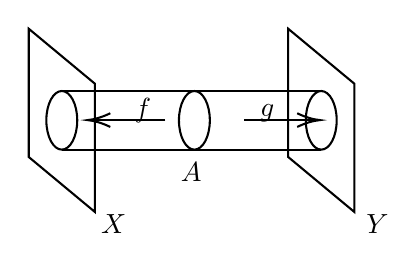
\begin{tikzpicture}[x=0.75pt,y=0.75pt,yscale=-1,xscale=1]
			%uncomment if require: \path (0,300); %set diagram left start at 0, and has height of 300
			
			%Shape: Parallelogram [id:dp15297514694080894] 
			\draw   (96.58,101.28) -- (96.58,163.07) -- (64.71,136.59) -- (64.71,74.8) -- cycle ;
			%Shape: Ellipse [id:dp019834245813657114] 
			\draw   (73.2,118.93) .. controls (73.2,111.13) and (76.54,104.81) .. (80.65,104.81) .. controls (84.76,104.81) and (88.09,111.13) .. (88.09,118.93) .. controls (88.09,126.73) and (84.76,133.06) .. (80.65,133.06) .. controls (76.54,133.06) and (73.2,126.73) .. (73.2,118.93) -- cycle ;
			%Shape: Ellipse [id:dp40259616007577415] 
			\draw   (198.2,118.93) .. controls (198.2,111.13) and (201.54,104.81) .. (205.65,104.81) .. controls (209.76,104.81) and (213.09,111.13) .. (213.09,118.93) .. controls (213.09,126.73) and (209.76,133.06) .. (205.65,133.06) .. controls (201.54,133.06) and (198.2,126.73) .. (198.2,118.93) -- cycle ;
			%Shape: Parallelogram [id:dp06847355000424948] 
			\draw   (221.58,101.28) -- (221.58,163.07) -- (189.71,136.59) -- (189.71,74.8) -- cycle ;
			%Straight Lines [id:da049979386851016994] 
			\draw    (80.65,104.81) -- (205.65,104.81) ;
			%Straight Lines [id:da5162984256492849] 
			\draw    (80.65,133.06) -- (205.65,133.06) ;
			%Shape: Ellipse [id:dp7242785411673776] 
			\draw   (137.09,118.93) .. controls (137.09,111.13) and (140.42,104.81) .. (144.53,104.81) .. controls (148.64,104.81) and (151.97,111.13) .. (151.97,118.93) .. controls (151.97,126.73) and (148.64,133.06) .. (144.53,133.06) .. controls (140.42,133.06) and (137.09,126.73) .. (137.09,118.93) -- cycle ;
			%Straight Lines [id:da2856334310702111] 
			\draw    (130.5,118.83) -- (95.08,118.83) ;
			\draw [shift={(93.08,118.83)}, rotate = 360] [color={rgb, 255:red, 0; green, 0; blue, 0 }  ][line width=0.75]    (10.93,-3.29) .. controls (6.95,-1.4) and (3.31,-0.3) .. (0,0) .. controls (3.31,0.3) and (6.95,1.4) .. (10.93,3.29)   ;
			%Straight Lines [id:da6963451965198226] 
			\draw    (168.5,118.83) -- (203,118.83) ;
			\draw [shift={(205,118.83)}, rotate = 180] [color={rgb, 255:red, 0; green, 0; blue, 0 }  ][line width=0.75]    (10.93,-3.29) .. controls (6.95,-1.4) and (3.31,-0.3) .. (0,0) .. controls (3.31,0.3) and (6.95,1.4) .. (10.93,3.29)   ;
			
			% Text Node
			\draw (136.53,138) node [anchor=north west][inner sep=0.75pt]   [align=left] {$\displaystyle A$};
			% Text Node
			\draw (98.13,163) node [anchor=north west][inner sep=0.75pt]   [align=left] {$\displaystyle X$};
			% Text Node
			\draw (225.93,163) node [anchor=north west][inner sep=0.75pt]   [align=left] {$\displaystyle Y$};
			% Text Node
			\draw (114.25,107) node [anchor=north west][inner sep=0.75pt]   [align=left] {$\displaystyle f$};
			% Text Node
			\draw (174.75,110) node [anchor=north west][inner sep=0.75pt]   [align=left] {$\displaystyle g$};
		\end{tikzpicture}
	\end{center}
	
	同伦推出的例子可以启发一般的同伦余极限. 设 $T\colon I\to \mathsf {Top}$ 为拓扑空间的图表. 对指标范畴 $I$ 每个长为 $n$ 的态射链 $i_0\to i_1\to\cdots\to i_n$, 以及每个点 $a\in T(i_0)$, 普通的余极限会粗暴地将 $a$ 经过这些映射所到的每个点粘在一起, 而同伦余极限则是在这些点之间连上一个拓扑 $n$-单形 $|\Delta^n|$.
	具体地, 先由 $T$ 构造一个自然的单纯空间
	$\mathsf s T\colon \Delta^{\op} \to\mathsf {Top}$, 使得 $$\mathsf s T_n = \coprod_{i_0\to i_1\to\cdots\to i_n} T(i_0).$$
	对于单纯空间 $X\colon \Delta^{\op} \to\mathsf {Top}$, 定义其\emph{几何实现}为如下的余等化子,
	$$
	|X|:= \operatorname{coeq}\Big[
	\coprod_{[n]\to [k]} X_k\times |\Delta^n|
	\rightrightarrows
	\coprod_{n}X_n\times |\Delta^n|
	\Big]
	$$
	其中两个映射分别为
	$$
	\begin{aligned}
		\coprod_{\sigma\colon  [n] \to [k]}& (\sigma^*\colon X_k \to X_n)\times |\Delta^n|,\\
		\coprod_{\sigma\colon  [n] \to [k]}& X_k\times (|\sigma|\colon |\Delta^n|\to |\Delta^k|).
	\end{aligned}
	$$
	那么 $T$ 的\emph{同伦余极限}可构造为
	$$
	\operatorname{hocolim}T := |\mathsf sT|.
	$$
	
	同伦极限的一个例子是同伦拉回. 两个映射 $f\colon X\to A$, $g\colon Y\to A$ 的同伦拉回可构造为 $X\times A^{\mathbb I}\times Y$ 的子空间
	$$
	\big\{ (x,\gamma,y)\in X\times A^{\mathbb I}\times Y\mid  \gamma(0)=f(x),\gamma(1)=g(y)\big\}.
	$$
	同伦拉回中的一个点由 $X$ 的点 $x$, $Y$ 的点 $y$ 以及 $f(x)$ 到 $g(y)$ 的一条道路构成.
	\begin{center}
		\tikzset{every picture/.style={line width=0.75pt}} %set default line width to 0.75pt        
		
		
		\tikzset{every picture/.style={line width=0.75pt}} %set default line width to 0.75pt        
		
		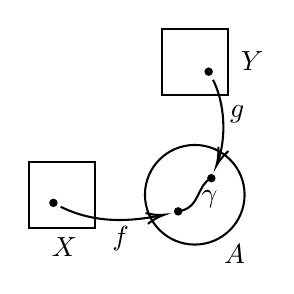
\begin{tikzpicture}[x=0.6pt,y=0.6pt,yscale=-1,xscale=1]
			%uncomment if require: \path (0,300); %set diagram left start at 0, and has height of 300
			
			%Shape: Square [id:dp9029850536154158] 
			\draw   (80,130) -- (120,130) -- (120,170) -- (80,170) -- cycle ;
			%Shape: Square [id:dp04010633466224678] 
			\draw   (160,50) -- (200,50) -- (200,90) -- (160,90) -- cycle ;
			%Shape: Circle [id:dp8217969120991764] 
			\draw   (150,150) .. controls (150,133.43) and (163.43,120) .. (180,120) .. controls (196.57,120) and (210,133.43) .. (210,150) .. controls (210,166.57) and (196.57,180) .. (180,180) .. controls (163.43,180) and (150,166.57) .. (150,150) -- cycle ;
			%Curve Lines [id:da9149134742462921] 
			\draw    (170,160) .. controls (183.75,158) and (180.75,144.25) .. (190,140) ;
			%Shape: Circle [id:dp3191495362532544] 
			\draw  [color={rgb, 255:red, 0; green, 0; blue, 0 }  ,draw opacity=1 ][fill={rgb, 255:red, 0; green, 0; blue, 0 }  ,fill opacity=1 ] (93,154.88) .. controls (93,153.84) and (93.84,153) .. (94.88,153) .. controls (95.91,153) and (96.75,153.84) .. (96.75,154.88) .. controls (96.75,155.91) and (95.91,156.75) .. (94.88,156.75) .. controls (93.84,156.75) and (93,155.91) .. (93,154.88) -- cycle ;
			%Shape: Circle [id:dp6370015580564639] 
			\draw  [color={rgb, 255:red, 0; green, 0; blue, 0 }  ,draw opacity=1 ][fill={rgb, 255:red, 0; green, 0; blue, 0 }  ,fill opacity=1 ] (186.5,75.88) .. controls (186.5,74.84) and (187.34,74) .. (188.38,74) .. controls (189.41,74) and (190.25,74.84) .. (190.25,75.88) .. controls (190.25,76.91) and (189.41,77.75) .. (188.38,77.75) .. controls (187.34,77.75) and (186.5,76.91) .. (186.5,75.88) -- cycle ;
			%Shape: Circle [id:dp21083479803073035] 
			\draw  [color={rgb, 255:red, 0; green, 0; blue, 0 }  ,draw opacity=1 ][fill={rgb, 255:red, 0; green, 0; blue, 0 }  ,fill opacity=1 ] (168.13,160) .. controls (168.13,158.96) and (168.96,158.13) .. (170,158.13) .. controls (171.04,158.13) and (171.88,158.96) .. (171.88,160) .. controls (171.88,161.04) and (171.04,161.88) .. (170,161.88) .. controls (168.96,161.88) and (168.13,161.04) .. (168.13,160) -- cycle ;
			%Shape: Circle [id:dp6826214678369391] 
			\draw  [color={rgb, 255:red, 0; green, 0; blue, 0 }  ,draw opacity=1 ][fill={rgb, 255:red, 0; green, 0; blue, 0 }  ,fill opacity=1 ] (188.13,140) .. controls (188.13,138.96) and (188.96,138.13) .. (190,138.13) .. controls (191.04,138.13) and (191.88,138.96) .. (191.88,140) .. controls (191.88,141.04) and (191.04,141.88) .. (190,141.88) .. controls (188.96,141.88) and (188.13,141.04) .. (188.13,140) -- cycle ;
			%Curve Lines [id:da8630666727441021] 
			\draw    (99.25,157.25) .. controls (118.75,166.76) and (138.49,166.76) .. (160.08,162.35) ;
			\draw [shift={(161.75,162)}, rotate = 167.95] [color={rgb, 255:red, 0; green, 0; blue, 0 }  ][line width=0.75]    (10.93,-3.29) .. controls (6.95,-1.4) and (3.31,-0.3) .. (0,0) .. controls (3.31,0.3) and (6.95,1.4) .. (10.93,3.29)   ;
			%Curve Lines [id:da25052543255059834] 
			\draw    (191,80.75) .. controls (198,94.5) and (199.41,115.47) .. (193.65,130.85) ;
			\draw [shift={(193,132.5)}, rotate = 292.75] [color={rgb, 255:red, 0; green, 0; blue, 0 }  ][line width=0.75]    (10.93,-3.29) .. controls (6.95,-1.4) and (3.31,-0.3) .. (0,0) .. controls (3.31,0.3) and (6.95,1.4) .. (10.93,3.29)   ;
			
			% Text Node
			\draw (195.75,178) node [anchor=north west][inner sep=0.75pt]   [align=left] {$\displaystyle A$};
			% Text Node
			\draw (92,174) node [anchor=north west][inner sep=0.75pt]   [align=left] {$\displaystyle X$};
			% Text Node
			\draw (206,62) node [anchor=north west][inner sep=0.75pt]   [align=left] {$\displaystyle Y$};
			% Text Node
			\draw (128.5,167) node [anchor=north west][inner sep=0.75pt]   [align=left] {$\displaystyle f$};
			% Text Node
			\draw (199.5,94.5) node [anchor=north west][inner sep=0.75pt]   [align=left] {$\displaystyle g$};
			% Text Node
			\draw (182.25,145.75) node [anchor=north west][inner sep=0.75pt]   [align=left] {$\displaystyle \gamma $};
			
			
		\end{tikzpicture}
	\end{center}
	一般地, 设 $T\colon I\to \mathsf {Top}$ 为拓扑空间的图表, 对指标范畴 $I$ 每个长为 $n$ 的态射链 $i_0\to i_1\to\cdots\to i_n$, 以及每个点 $a\in T(i_n)$, 普通的极限只允许 $T(i_0),\cdots,T(i_n)$ 的各点恰好落在 $a$ 上, 而同伦极限允许它们落在 $T(i_n)$ 中的一个 $n$-单形的顶点. 具体地, 构造自然的余单纯空间 $\mathsf cT\colon \Delta \to \mathsf {Top}$, 使得
	$$
	\mathsf cT_n = \prod_{i_0\to \cdots\to i_n} T(i_n).
	$$
	对于余单纯空间 $X\colon \Delta\to\mathsf {Top}$, 定义其\emph{全体} (totalization)\footnotemark{} $\operatorname{Tot}X$ 为如下的等化子,
	$$
	\operatorname{Tot}X := \operatorname{eq}\Big[
	\prod_{n}X_n^{|\Delta^n|}
	\rightrightarrows
	\prod_{[n]\to [k]} X_k^{|\Delta^n|}
	\Big].
	$$
	
	同伦极限和同伦余极限\emph{表现}了 $\infty$-范畴中的极限和余极限. 见 \cite{HTT} 定理 4.2.4.1.
\end{remark}
\footnotetext{几何实现是一种左 Kan 扩张, 而 ``全体'' 是一种右 Kan 扩张. 记 $\mathsf{cosTop}$ 为余单纯空间的范畴, 则余单纯空间 $X$ 的全体也可表示为 $\operatorname{Hom}_{\mathsf{cosTop}}(|\Delta|,X)$, 其中 $|\Delta|\colon \Delta\to \mathsf {Top}$ 将 $[n]$ 对应到拓扑 $n$-单形.}

\begin{example}
	{}
	对于 $I = \varnothing$, 空图表 $F\colon I\to \mathcal C$ 的极限即是 $\mathcal C$ 的终对象.
\end{example}

\begin{example}
	{(推出, 拉回)}
	考虑 $I = \Lambda_2^2$ (见定义 \ref{simplicial-set-horn} 及其后的插图), 则 $F\colon I\to X$ 等同于两个态射 $x\to z$, $y\to z$. 称 $F$ 的极限为 $\infty$-\emph{拉回}, 简称\emph{拉回}, 记为 $x\times_z y$.
	对偶地, 形如 $\Lambda_0^2$ 的图的余极限称为 $\infty$-\emph{推出}, 简称\emph{推出}.
	
	单纯集映射 % https://q.uiver.app/#q=WzAsMyxbMCwwLCJYIl0sWzEsMCwiWSJdLFswLDEsIloiXSxbMCwyXSxbMCwxXV0=
	$\begin{tikzcd}[ampersand replacement=\&,sep=small]
		X \& Y \\
		Z
		\arrow[from=1-1, to=2-1]
		\arrow[from=1-1, to=1-2]
	\end{tikzcd}$ 的\emph{同伦推出}为 $Y\sqcup_{\{0\}\times X}(\Delta^1\times X)\sqcup_{\{1\}\times X}Z$.
\end{example}

\begin{definition}
	{(环路空间)}
	
\end{definition}


\subsection{$\operatorname{Hom}$ 函子, 预层与 $\infty$-米田引理}

\philoquote{Perhaps the main technical challenge in extending classical categorical results to the $\infty$-categorical context is in merely \emph{defining} the Yoneda embedding.}{Emily Riehl \& Dominic Verity,\\\emph{The Comprehension Construction}}

我们希望定义 $\infty$-版本的预层范畴, 并建立米田引理. 参考卷 1 注 \ref{t1-Yoneda-embedding-adjoint-Hom}, 我们首先需要一个函子 $\operatorname{Hom}\colon \mathcal C^\op\times\mathcal C\to \infGpdinfcat$. 这个函子同样可借助单纯范畴构造. 注意这并非 $\infty$-范畴理论中陈述米田引理的唯一方法.


\begin{definition}
	{(预层 $\infty$-范畴)}
	设 $\mathcal C$ 为 $\infty$-范畴. 定义 $$\widehat {\mathcal C} := \mathsf {Fun}(\mathcal C^\op,\infGpdinfcat)$$
	为 $\mathcal C$ 上的\emph{预层 $\infty$-范畴}.
\end{definition}

\begin{prop}
	{}
	
\end{prop}

\todo{自由余完备化}

%\section{$\infty$-范畴: 公理化}




% https://ncatlab.org/nlab/show/(0,1)-category

% 介绍 (0,1)-topos = Heyting algebra

\todo{}

%\section{$\infty$-层 $\infty$-\topos{}及其表现}
%
%$\infty$-层是层在 $\infty$-范畴中的类比. 正如层构成\topos{}, $\infty$-层也构成 $\infty$-\topos{}.
%
%% https://ncatlab.org/nlab/show/presentations+of+%28infinity%2C1%29-sheaf+%28infinity%2C1%29-toposes
